\documentclass[a4paper,12pt]{report}
\usepackage{titlesec}
\usepackage{tocloft} % pour la table des matières
\usepackage{pdfpages}
\usepackage[utf8]{inputenc}
\usepackage[backend=biber]{biblatex}
\addbibresource{biblio.bib}
\usepackage{hyperref}
\usepackage{abstract} % nous on a un abstract
\usepackage{tabularx}
\usepackage{graphicx}
\usepackage{xcolor}
\usepackage{array}
\usepackage{float}
\usepackage{amsmath}
\usepackage{multirow}
\usepackage{appendix}
\usepackage{adjustbox}
\usepackage{fancyhdr}
\usepackage{listings}
\usepackage{import}
\usepackage[nottoc,numbib]{tocbibind} %adding the bib to toc
\usepackage{rotating} %pour les tableaux
\usepackage{enumitem} % pour citer (mettre des tirets etc)
\usepackage[nounderscore]{syntax}
\usepackage[T1]{fontenc}
\usepackage[french]{babel} %comme ça tout tes list of figures deviendront direct en francais tables des
\usepackage[french]{nomencl}
\usepackage{xcolor,graphicx}
\newcounter{insertpages}
\usepackage[automake]{glossaries} %liste des abréviations
%\usepackage[acronym]{glossaries}
\graphicspath{{image/}} %path de tes images
\newcommand{\RomanNumeralCaps}[1]
{\MakeUppercase{\romannumeral #1}}
\usepackage[top=2cm, bottom=2cm, left=3cm, right=2cm]{geometry} % dimension de la page
\linespread{1.5}
\newenvironment{poliabstract}[1]
  {\renewcommand{\abstractname}{#1}\begin{abstract}}
  {\end{abstract}} %abstract sur 2 pages

\renewcommand{\acronymname}{Listes des abréviations}

\makeglossaries
%\newglossaryentry{maths}
%{
    %name=mathematics,
    %description={Mathematics is what mathematicians do}
%}


%%%%% style pour le code %%%%


% Definig a custom style:
\lstdefinestyle{mystyle}{
    backgroundcolor=\color{white},   
    commentstyle=\color{purple},
    keywordstyle=\color{blue},
    numberstyle=\tiny\color{gray},
    stringstyle=\color{purple},
    basicstyle=\ttfamily\footnotesize\bfseries,
    breakatwhitespace=false,         
    breaklines=true,                 
    captionpos=t,                    
    keepspaces=false,                 
    numbers=left,                    
    numbersep=5pt,                  
    showspaces=false,                
    showstringspaces=false,
    showtabs=false,                  
    tabsize=2
}

% -- Setting up the custom style:
\lstset{style=mystyle}

\lstset{
  style=mystyle,
%  frame= single,
%  linewidth=0.6\linewidth,
%  xleftmargin=12pt,
%  aboveskip=12pt,
%  belowskip=12pt
}

%%%%%%%%%%%%%%%%%%



\loadglsentries{liste des abréviations}



\begin{document}
\renewcommand{\listfigurename}{Table des figures}
\newpage
\renewcommand{\listtablename}{Listes des tableaux}
\newpage
%\renewcommand\appendixpagename{Annexe}

\pagenumbering{gobble}


\includepdf[pages={1}]{COUVERTURE.pdf} %car je ne peux pas inclure un fichier qui n'est pas déjà compilé

\null\newpage %saut de page

%\renewcommand*\contentsname{Sommaire}
%\includepdf[pages={1}]{couverture.pdf}
\tableofcontents{} %table des matières
%\include{Cahier des charges}

\pagenumbering{roman} %numérotation des pages


\listoffigures{}
\null\newpage
%\vspace{6cm}
\listoftables{}

%\printglossary[title={Nomenclature}]
%\addcontentsline{toc}{chapter}{Nomenclature}
%\vspace{7cm}
%\input{Liste des abréviations}








%% gesticulation c'est le header en haut 
\pagestyle{fancy}
\fancyhead{} % clear all header fields
\fancyhead[LO,CE]{Distributeur intelligent d'aliments pour chat}
\fancyhead[RO,LE]{2024-2025}
%\fancyfoot[C]{\thepage} % Exemple footer
%\renewcommand{\footrulewidth}{1pt} %  ligne pour le footer


 %prend le fichier .tex l'ajoute à la compilation
%\input{généralités}
%\input{ETUDE ET CONCEPTION}
%\input{REALISATION ET ESSAIS}
%\input{CONCLUSION GENERALE}

%pour afficher la bilbio
\nopagebreak
\printbibliography[heading=bibintoc,type=misc,title={Bibliographie}] 
 
\pagenumbering{Roman}
\setcounter{page}{8}
\nopagebreak
\printbibliography[heading=bibintoc,type=online,title={Webographie}]
\nopagebreak
\nopagebreak[4]
\addappheadtotoc
%\clearpage
%\include{ANNEXE}
%\printglossary[title=Glossaire, toctitle=Glossaire]
\null\newpage
%\renewcommand*\contentsname{Table des matières}
%\tableofcontents{} %table des matières
%\include{Cahier des charges}
\chapter{Description du projet}
\addcontentsline{toc}{chapter}{Description du projet}
\section{Formulation}
Ce projet consiste à concevoir un distributeur automatique de nourriture pour chat, qui peut être contrôlé à distance via une application mobile. 
\section{Objectif du projet}
	L'objectif est de permettre aux propriétaires de chats de nourrir leurs animaux même lorsqu'ils sont absents, en programmant des horaires et des quantités de nourriture à distribuer. Le système doit également offrir des fonctionnalités de contrôle manuel, de notifications et d'historique des distributions.
\section{Besoins des utilisateurs}

Voici la liste des besoins des utilisateurs :

\begin{itemize}
	\item Planification des repas : Les utilisateurs devraient pouvoir définir à l'avance les horaires et les quantités de nourriture à distribuer.
	\item Distribution manuelle : Il est important de permettre aux utilisateurs de distribuer de la nourriture à la demande via l'application, en dehors des horaires programmés.
	\item Notifications : des alertes devraient être générées lorsque la nourriture est distribuée ou lorsque le niveau de nourriture est bas, afin de rester informés en temps réel.
	\item Historique des distributions : Un suivi des distributions pour que les utilisateurs puissent consulter les repas précédemment servis.
	\item Sécurité des accès : une authentification sécurisée pour éviter tout accès non autorisé à l'application.
	\item Réglage des quantités : permettre aux utilisateurs de définir précisément la quantité de nourriture à distribuer à chaque repas.
\end{itemize}
    
\section{Moyen nécessaire à la réalisation du projet}
	\subsection{Moyens Matériel}
	Pour réaliser ce projet, on aura besoin des éléments suivants :
		\begin{itemize}
			\item \textit{1 microcontrôleur ESP32} pour la connectivité Wi-Fi et le contrôle des composants.
			\item \textit{1 servo-moteur} pour contrôler la distribution de la nourriture.
			\item \textit{2 capteurs de poids} permettant de mesurer la quantité de nourriture distribuée ainsi que le reste de nourriture dans le reservoir.
			\item \textit{Des bois et des vis} pour assembler le distributeur.
			\item \textit{2 LED} pour indiquer l'état du distributeur (distribution en cours, niveau de nourriture bas).
		\end{itemize}
	\subsection{Moyens Logiciel}
	Pour le développement du logiciel, les outils suivants seront nécessaires :
		\begin{itemize}
			\item \textit{IDE Arduino} : pour la programmation de l'ESP32.
			\item \textit{Android Studio} : pour le développement de l'application mobile.
			\item \textit{Firebase Realtime Database} : pour le stockage des données des utilisateurs et des configurations de distribution.
			\item \textit{Serveur web} : pour gérer les requêtes entre l'ESP32 et la base de données.
			\item \textit{Git} : pour la gestion des versions du code source.
			\item \textit{WokWi} : pour la simulation des comportements des matériels éléctroniques.
			\item \textit{LatexMaker} : pour la rédaction du rapport de projet.
		\end{itemize}
	
		\subsection{Moyens Humains}
	Pour la réalisation de ce projet, une équipe de 4 personnes est nécessaire, avec les rôles suivants :
		\begin{itemize}
			\item \textbf{2 développeurs} : responsables de la programmation de l’ESP32, de l’intégration des capteurs et du développement des communications WebSocket.
			\item \textbf{2 développeurs} : chargés de la conception et du développement de l’application mobile.
		\end{itemize}

\pagenumbering{arabic}
\setcounter{page}{1}       






\pagestyle{fancy}
\fancyhead{} % clear all header fields
\fancyhead[LO,CE]{Conception logicielle}
\fancyhead[RO,LE]{2024-2025}
\chapter{Conception logicielle}
\section{Architecture système}
L’application suit une architecture modulaire basée sur le MVVM(modèle-vue-vue modèle), divisée en trois couches principales :

\begin{itemize}
\item    Présentation (UI) : Gérée par des Composants Jetpack Compose et des ViewModels.
\item    Domain (Métier) : Contient les Use Cases et les interfaces de Repository.
\item    Data (Accès aux données) : Implémente les sources de données (Firebase, ESP32, Capteurs).
\end{itemize}
L'application communique directement avec Firebase pour la gestion des données, afin de transmettre à l'ESP32 les paramètres de configuration. La figure~\ref{fig:architecture_systeme} illustre cette architecture.

\begin{figure}[H]
   \centering
   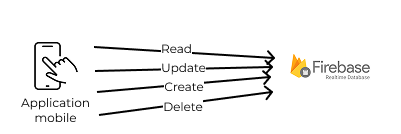
\includegraphics[scale=1]{archi_firebase.png}
   \caption{Communication entre l'application mobile et firebase}
   \label{fig:structure_de_la_base_de_donnees}
\end{figure}

\section{Structure de la base de données dans Realtime Database}

L'application utilise une base de données de type \textit{clé-valeur} appelée \textbf{Realtime Database}, hébergée et gérée par Firebase. Cette base de données offre plusieurs avantages, tels qu'une infrastructure sans serveur, une haute disponibilité et une sécurité assurée par Google. La structure des données utilisée est illustrée à la figure~\ref{fig:structure_de_la_base_de_donnees}.

\begin{figure}[H]
   \centering
   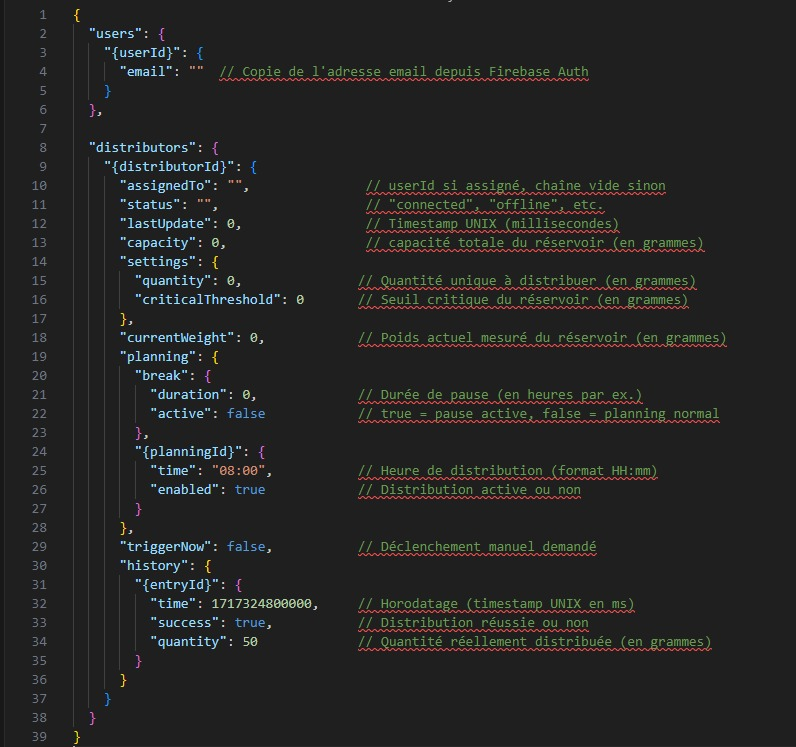
\includegraphics[scale=0.5]{dd3.jpeg}
   \caption{Structure de la base de données}
   \label{fig:structure_de_la_base_de_donnees}
\end{figure}

La base de données contient deux clés principales :

\begin{itemize}
\item \textbf{users} : contient les informations de tous les utilisateurs de l'application mobile.
\item \textbf{distributors} : contient les paramètres des distributeurs automatiques de nourriture pour chats.
\end{itemize}

\begin{enumerate}[label=\alph*)]
\item \textbf{Données des utilisateurs} 

\textbf{Firebase Authentication} est utilisé pour gérer l'authentification des utilisateurs. Les informations d'authentification sont stockées et gérées par ce service. Les données spécifiques à chaque utilisateur, stockées dans Realtime Database, sont :

\begin{itemize}
\item \textbf{\{userId\}} : identifiant unique généré par Firebase Authentication pour chaque utilisateur.
\item \textbf{email} : adresse e-mail utilisée par l'utilisateur pour se connecter à l'application.
\end{itemize}

\item \textbf{Données des distributeurs} 

Les données des distributeurs servent principalement à configurer leurs actions. Ces données incluent :

\begin{itemize}
\item \textbf{\{distributorId\}} : identifiant unique de chaque distributeur, généré lors de l'assemblage du matériel.
\item \textbf{assignedTo} : identifiant de l'utilisateur associé au distributeur.
\item \textbf{status} : état de la connexion Internet de l'ESP32.
\item \textbf{lastUpdate} : date de la dernière activité du distributeur.
\item \textbf{capacity} : capacité totale du réservoir en grammes.
\item \textbf{settings} : paramètres de distribution des croquettes, comprenant :
  \begin{itemize}
    \item \textit{quantity} : quantité à distribuer en grammes.
    \item \textit{criticalThreshold} : seuil critique du réservoir en grammes.
  \end{itemize}
\item \textbf{currentWeight} : poids actuel mesuré du réservoir en grammes.
\item \textbf{planning} : liste des distributions programmées par l'utilisateur. Chaque entrée contient :
  \begin{itemize}
    \item \textit{time} : heure de distribution au format \textit{HH:mm}.
    \item \textit{enabled} : indique si la distribution est active.
    \item \textit{break} : indique une pause dans la distribution.
  \end{itemize}
\item \textbf{triggerNow} : booléen indiquant un déclenchement manuel du distributeur.
\item \textbf{history} : historique des distributions effectuées.
\end{itemize}



\end{enumerate}

\section{Fonctionnalités clés de l’application} 
\begin{itemize}
	\item \textbf{Gestion des utilisateurs (Firebase Auth)} : 
	L'inscription et la connexion se font via email et mot de passe. Seul l’utilisateur authentifié peut accéder à son distributeur et le contrôler, garantissant ainsi une sécurité des accès.

	\item \textbf{Programmation des repas} :
	Les utilisateurs peuvent planifier les horaires et les quantités de nourriture à distribuer. Ces informations sont enregistrées dans Firebase avec \textbf{Real Time Database}.

	\item \textbf{Contrôle manuel} :
	Il est possible de déclencher manuellement une distribution de nourriture via l’application. Une commande est envoyée depuis Firebase, ce qui active un "trigger" de type booléen sur l’ESP32, permettant de lancer immédiatement une distribution.

	\item \textbf{Notifications} :
	L’utilisateur reçoit des alertes depuis l’application mobile, comme la confirmation qu’un repas a bien été distribué ou un avertissement en cas de niveau de nourriture bas. Ces notifications sont générées par un "trigger" associé aux événements dans l’application.

	\item \textbf{Historique des distributions} :
	Toutes les distributions, automatiques ou manuelles, sont enregistrées. L’utilisateur peut ainsi consulter l’historique des repas déjà servis, directement depuis l’application.

	\item \textbf{Réglage des quantités} :
	Pour chaque distribution, l’utilisateur peut définir précisément la quantité de nourriture à délivrer, en fonction des besoins de l’animal.
\end{itemize}


\pagestyle{fancy}
\fancyhead{} % clear all header fields
\fancyhead[LO,CE]{Conception électronique}
\fancyhead[RO,LE]{2024-2025}
\chapter{Conception électronique}
\section{Présentation matériel}
Ce projet a comme partie électronique les composants suivant : pour le microcontrôleur nous avons utilisés l'ESP32, 2 capteurs de poids avec muni convertisseur analogique vers numérique de 24 bits le HX711, et d'un servomoteur.

\begin{itemize}
\item \underline{\textbf{le microcontrôleur}:} L’ESP32 est un microcontrôleur à faible consommation d’énergie, doté d’un processeur double cœur 32 bits, de connexions Wi-Fi et Bluetooth intégrées. Il est largement utilisé pour les projets IoT (Internet des Objets) grâce à sa puissance de calcul, sa connectivité sans fil, ses nombreux broches. Pour ce projet, le dispositif est doté de l'ESP32 WROOM-32 DevKit à 38 broches.\\


\begin{figure}[H]
	\centering
	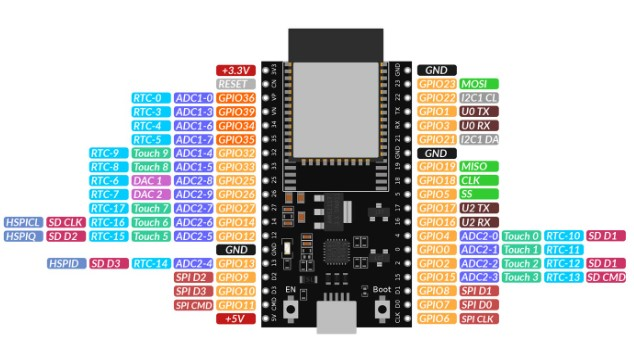
\includegraphics[scale=0.8]{1.jpg}
	\caption{Brochage de l'ESP32 WROOM-32 DevKit}
\end{figure}

\item \underline{\textbf{les capteurs de poids}:} Ils utilisent des jauges de contrainte montées sur une cellule de charge pour détecter les déformations causées par une masse. Le HX711 est un convertisseur analogique-numérique (ADC) va amplifier et lire les signaux analogique de faible amplitude que va généré la cellule de charge. Ici, le dispositif utilise 2 capteurs de masse différentes l'un de 1kg et l'autre de 20kg pour le réservoir.

\begin{figure}[H]
	\centering
	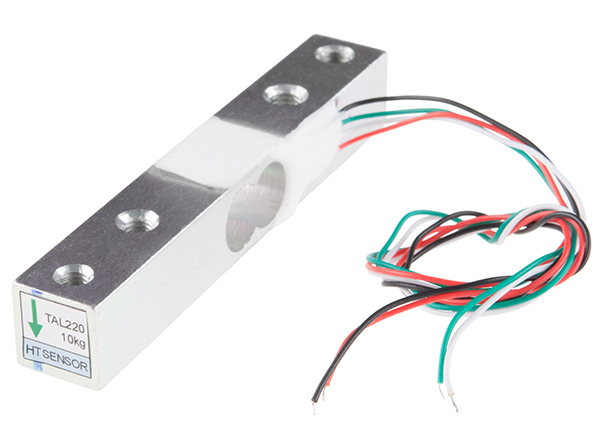
\includegraphics[scale=0.8]{2.jpg}
	\caption{Cellule de charge}
\end{figure}

\begin{figure}[H]
	\centering
	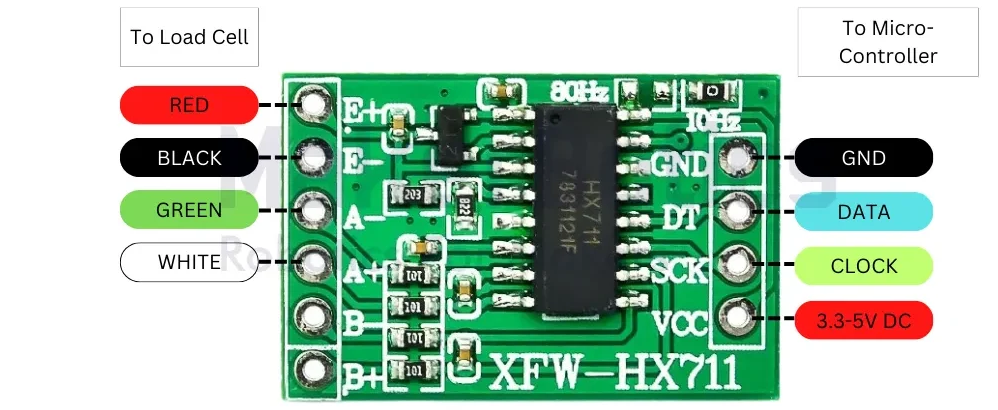
\includegraphics[scale=0.5]{1.png}
	\caption{Brochage du HX711}
\end{figure}

\item \underline{\textbf{le servo-moteur}:} C'est un moteur contrôlé en position, utilisé pour effectuer des rotations précises dans une plage définie (souvent 0° à 180°). Il reçoit un signal PWM (modulation de largeur d’impulsion), la largeur de l’impulsion détermine ainsi l’angle de rotation. Le servo-moteur servira d'ouverture de vanne dans notre cas.

\begin{figure}[H]
	\centering
	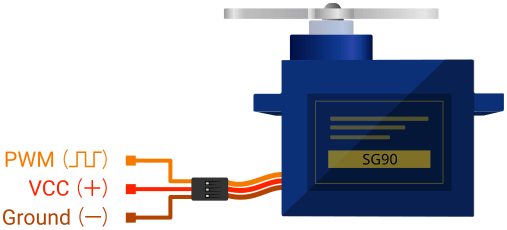
\includegraphics[scale=0.5]{2.png}
	\caption{Brochage du servo-moteur}
\end{figure}

\item  \underline{\textbf{Communication entre le microcontrôleur et le websocket}:} Pour récuperer les données depuis Firebase et le transmettre à l'ESP32, nous avons mis en place un serveur websocket, qui permet entre outre de recevoir des messages contenant des données depuis l'ESP32.  Le serveur websocket va ensuite les tranférer les données  vers  Real Time Database de Firebase.

\begin{figure}[H]
	\centering
	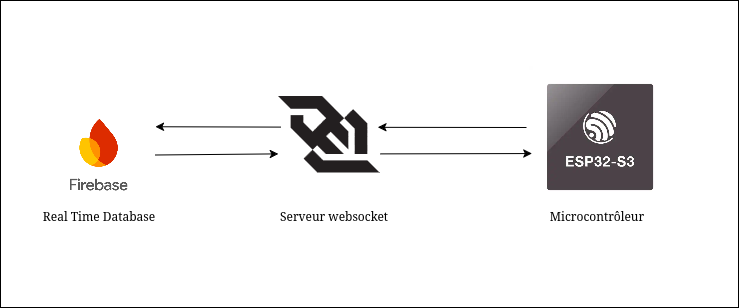
\includegraphics[scale=0.5]{4.png}
	\caption{Communication entre Firebase, le serveur websocket et l'ESP32}
\end{figure}

\end{itemize}


\section{Schéma d'ensemble du circuit}
Malheureusement, pas de beaucoup de logiciels peuvent simuler l'ESP32 et montrer précisement le schéma électronique du projet. Néanmoins, la platforme \textit{Wokwi}, permet cela, c'est une plateforme web qui permet de simuler à quelques détails près L'ESP32, et il nous fournit un schéma d'ensemble avec.\\[0.3cm]

\begin{figure}[H]
	\centering
	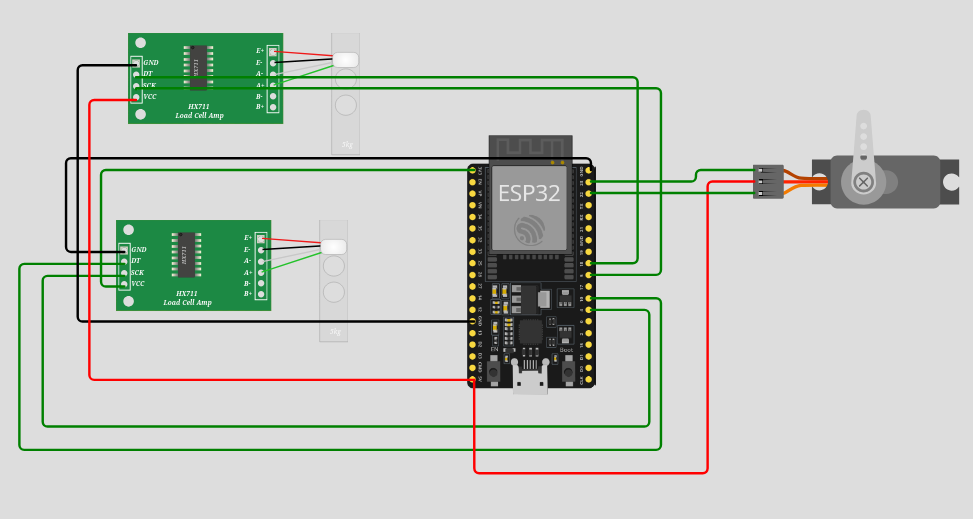
\includegraphics[scale=0.5]{3.png}
	\caption{Schéma d'ensemble du dispositif}
\end{figure}


\pagestyle{fancy}
\fancyhead{} % clear all header fields
\fancyhead[LO,CE]{Réalisation}
\fancyhead[RO,LE]{2024-2025}
\chapter{Réalisation}













\pagestyle{fancy}
\fancyhead{} % clear all header fields
\fancyhead[LO,CE]{Tests et validation}
\fancyhead[RO,LE]{2024-2025}
\chapter{Tests et validation}

\chapter*{Conclusion}
\addcontentsline{toc}{chapter}{Conclusion}

Ce projet alliant Kotlin (Android), ESP32 et Firebase illustre parfaitement comment les technologies modernes peuvent simplifier et améliorer le quotidien, même pour nos animaux de compagnie. Grâce à une architecture robuste (MVVM) et une synchronisation temps réel via Firebase, le système offre un contrôle intelligent qui permet une programmation précise des repas et distribution manuelle à distance. Une réactivité : le système de notifications instantanées et l'historique des distributions. Modularité une codebase claire (couches séparées) facilitant les évolutions futures. Accessibilité  une interface utilisateur intuitive (Jetpack Compose) et sécurisée (Firebase Auth).

Perspectives d’amélioration : 
\begin{itemize}

\item  Vision par caméra (ESP32-CAM) pour surveiller l’animal.

\item    Reconnaissance faciale (IA embarquée) pour personnaliser les repas.

\item    Optimisation énergétique avec mode veille et batterie de secours.
\end{itemize} 

Ce dispositif démontre aussi comment l’IoT et le mobile peuvent s’unir pour résoudre des problèmes concrets.

%\input{résumé}
%{\let\clearpage\relax\par \input{Abstract}} %mettre 2 chap sur une même page%

\end{document}
